\newpage
\section{Aufgabe3}
\label{sec:a3}

%
% \subsection{a)}
% \label{subsec:a3a}
% \begin{figure}
%   \centering
%   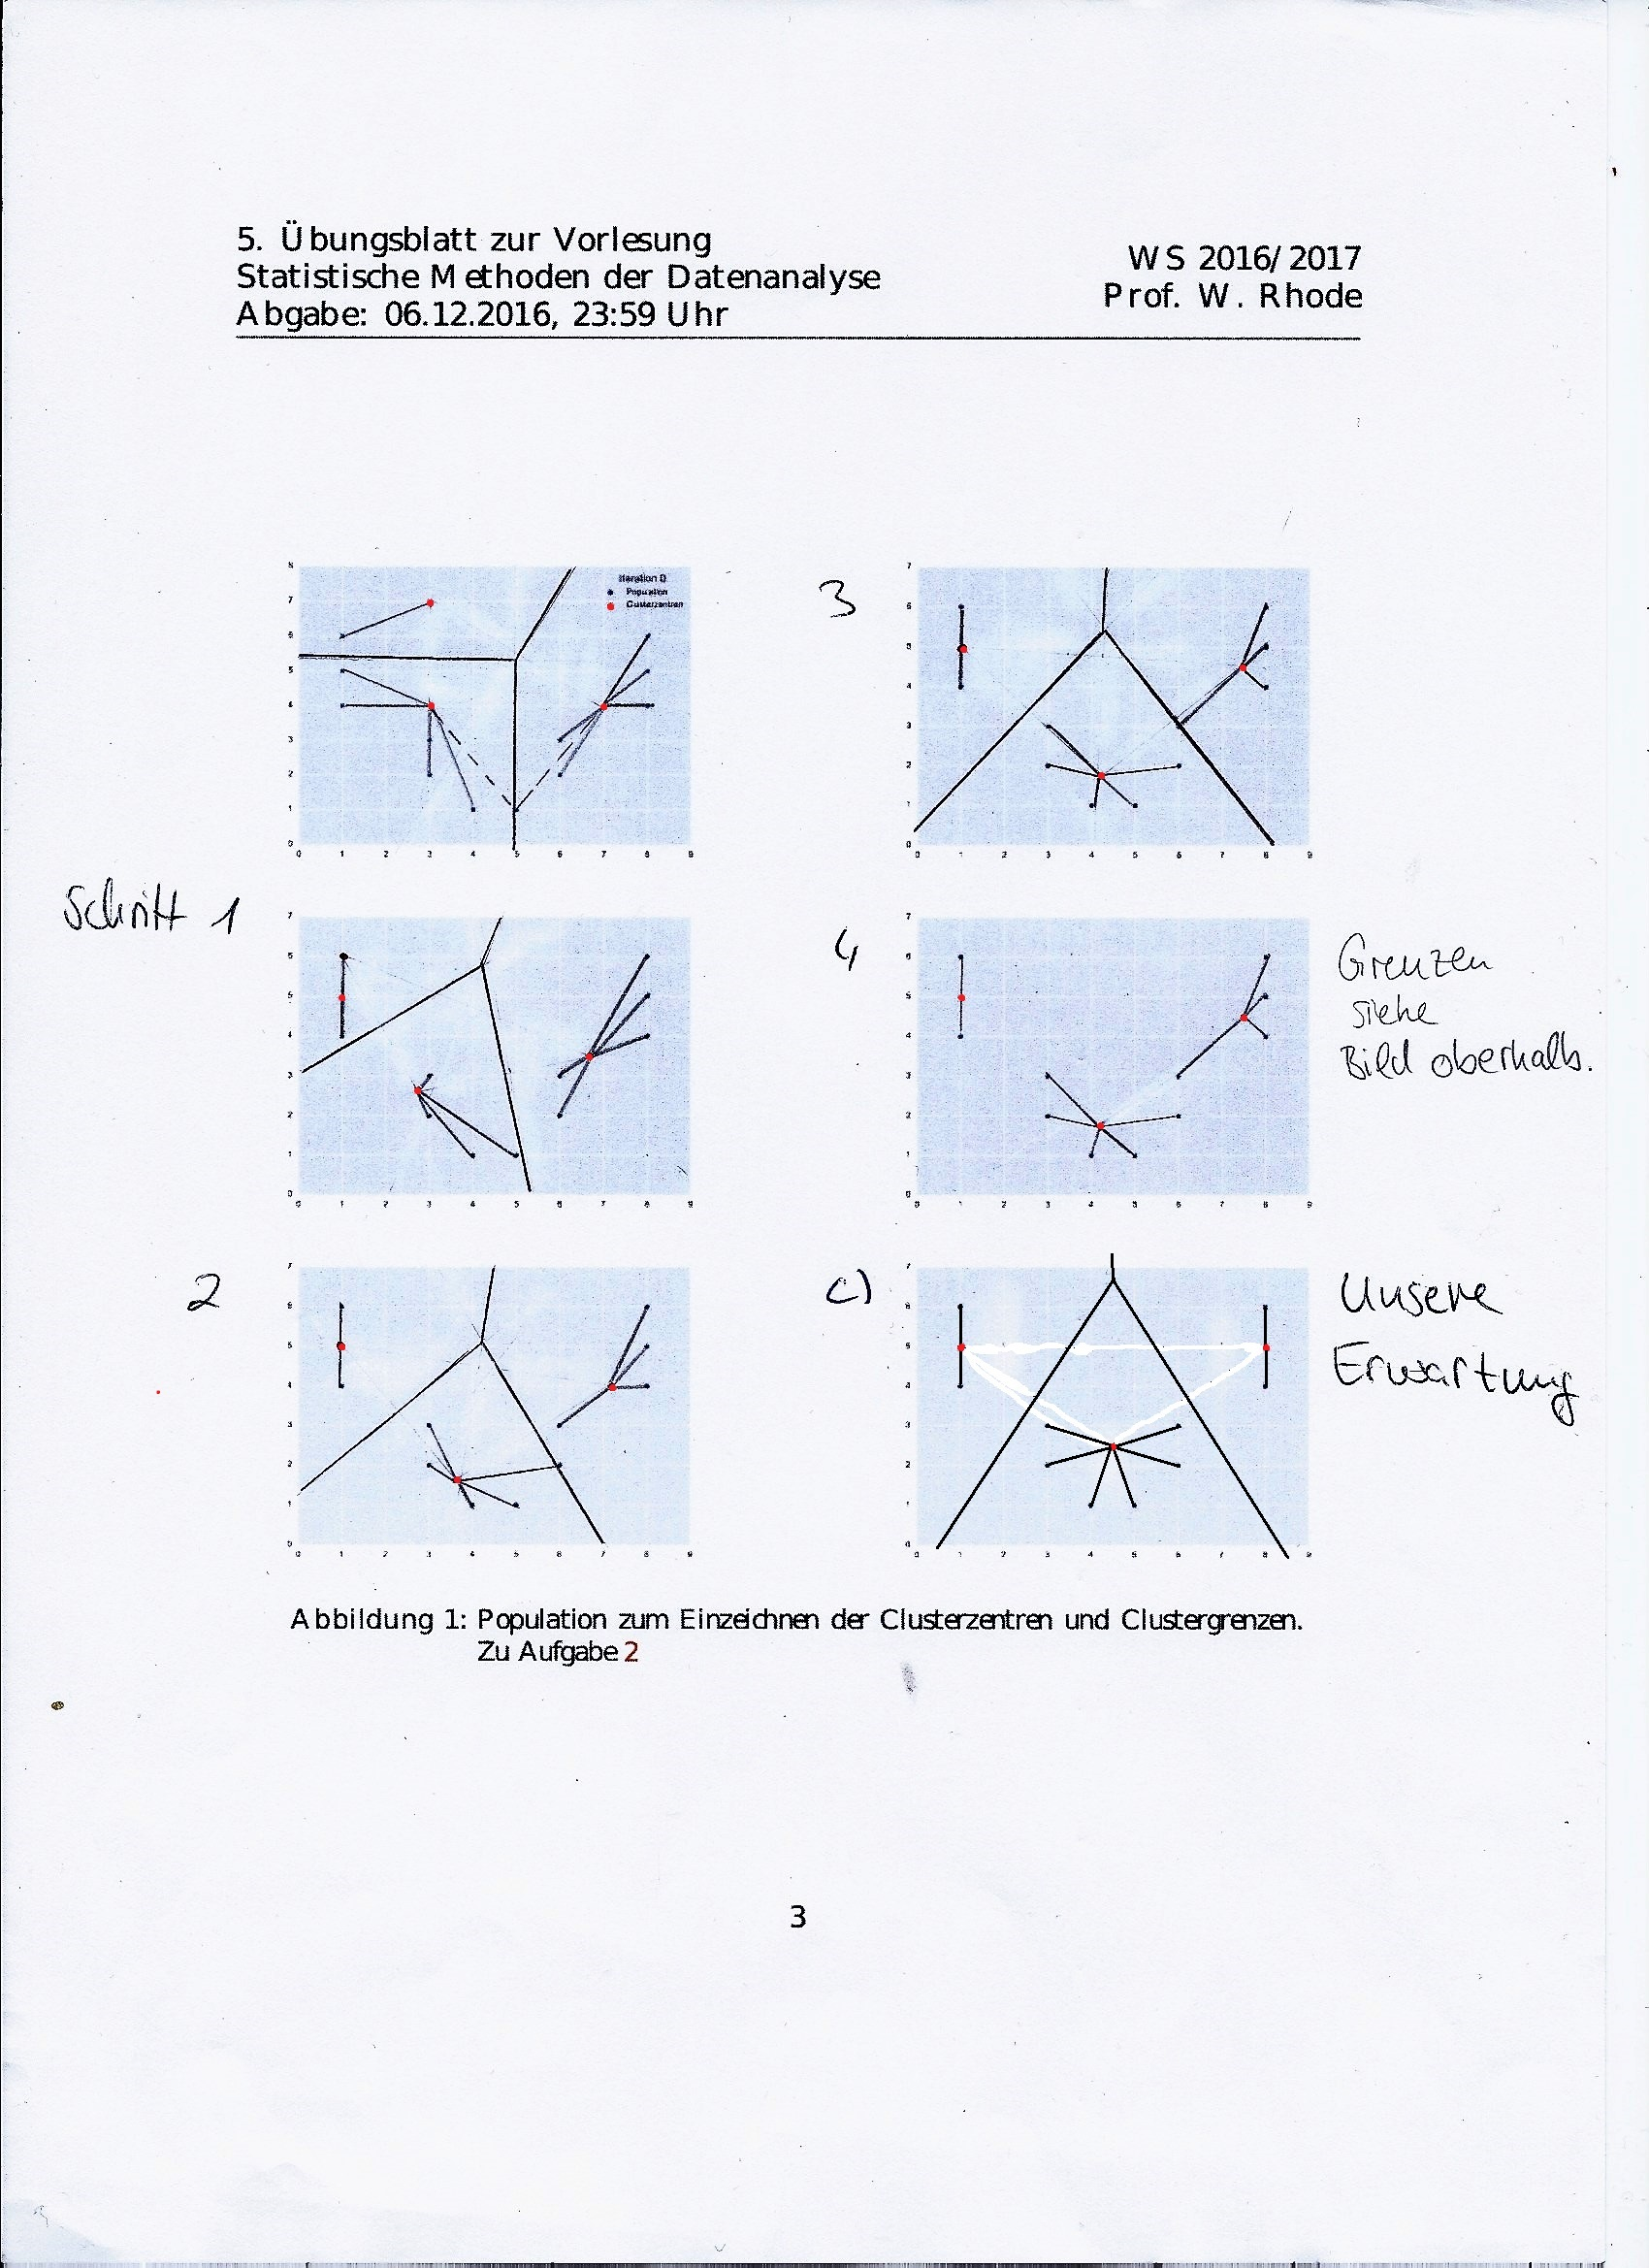
\includegraphics[width=\textwidth]{PhotoScan1.jpg}
%   \caption{}.
%   \label{fig:1}
% \end{figure}


\subsection{b)}
\label{subsec:a3b}



\subsection{c)}
\label{subsec:a3c}

In den Abbildungen \ref{fig:Temperatur}- \ref{fig:Luftfeuchigkeit}
ist der Informationsgewinn
in Abbhängigkeit der jeweiligen Schnitte auf den
unterschiedlichen Attributen aufgetragen.


\begin{figure}
  \centering
  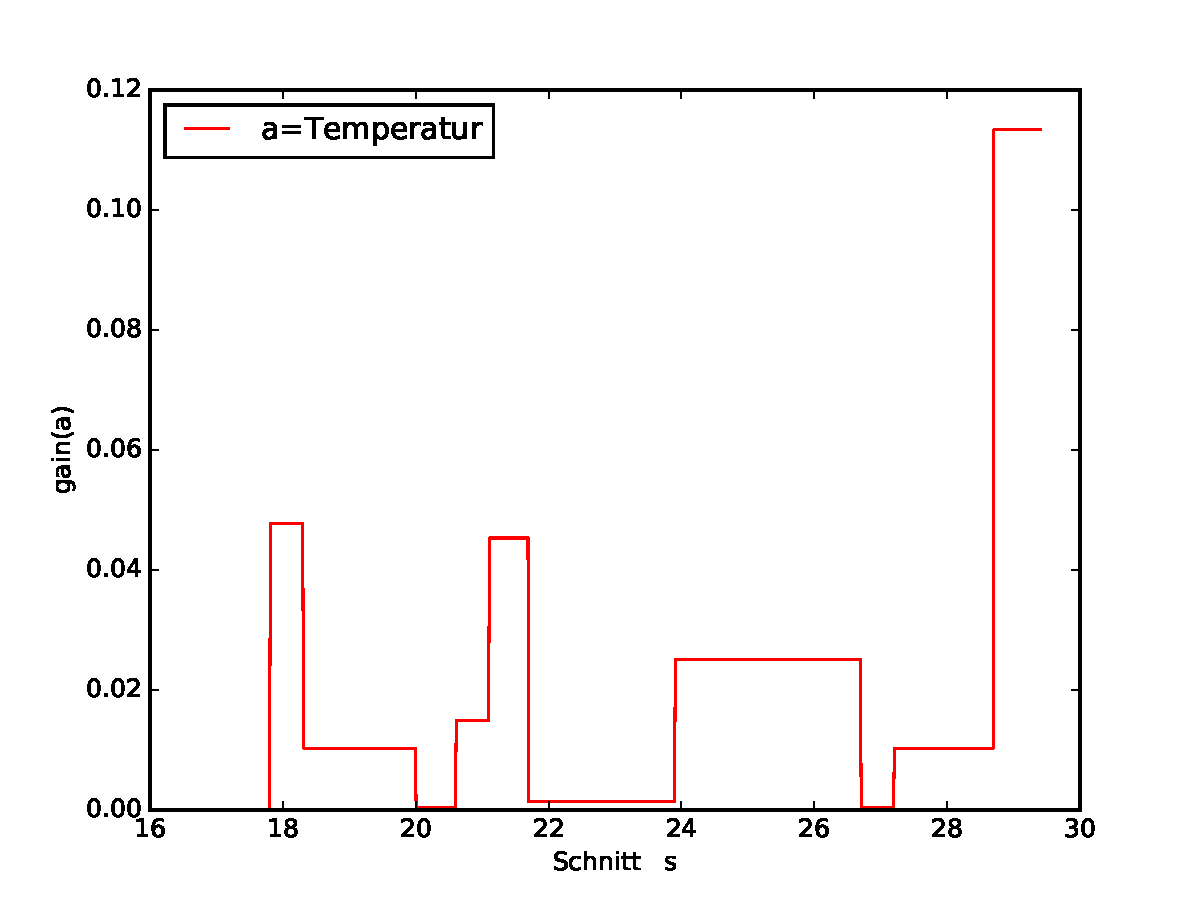
\includegraphics[width=0.7\textwidth]{Temperatur.pdf}
  \caption{ Der Informationsgewinn gain(a) in Abhängigkeit von dem Schnitt $s$ auf dem Attribut a=Temperatur .}
  \label{fig:Temperatur}
\end{figure}


\begin{figure}
  \centering
  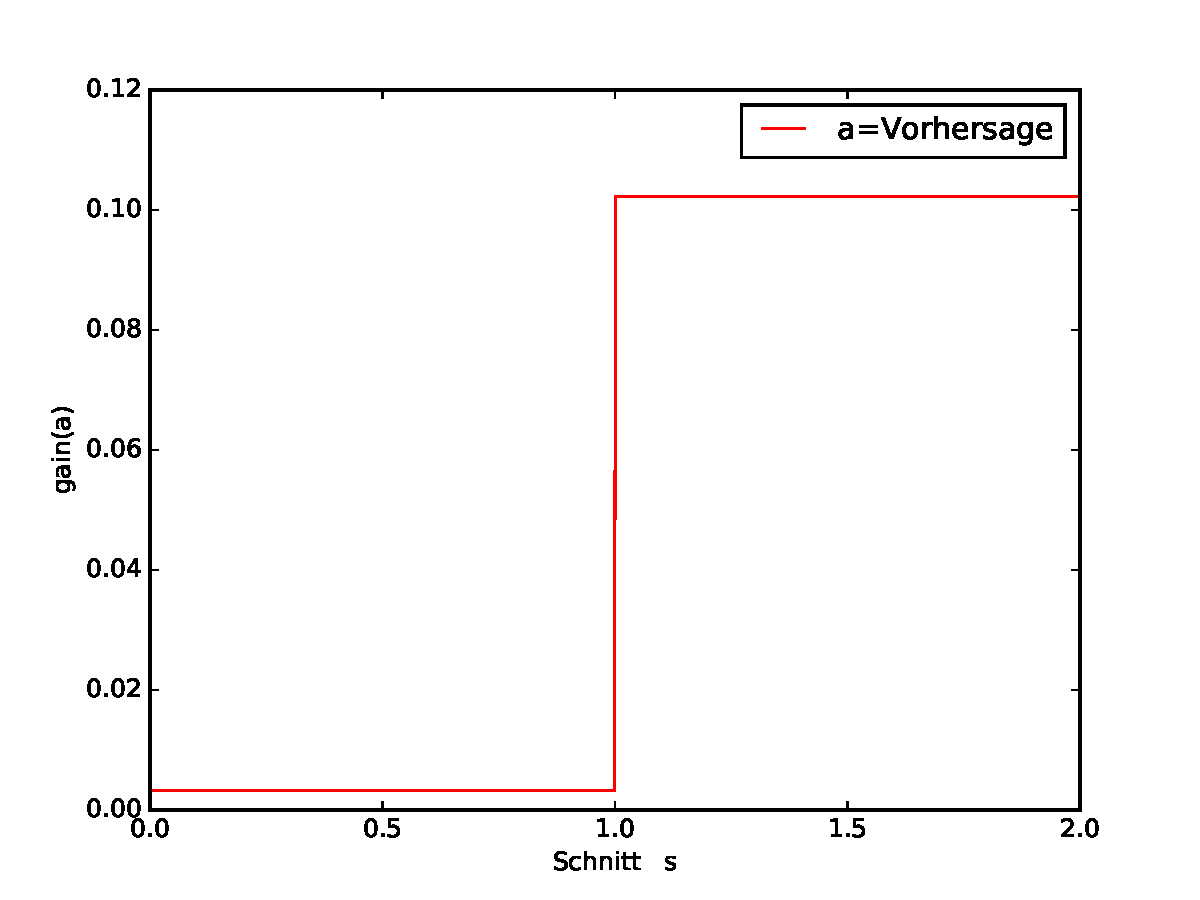
\includegraphics[width=0.7\textwidth]{Vorhersage.pdf}
  \caption{ Der Informationsgewinn gain(a) in Abhängigkeit von dem Schnitt $s$ auf dem Attribut a=Wettervorhersage .}
  \label{fig:Vorhersage}
\end{figure}


\begin{figure}
  \centering
  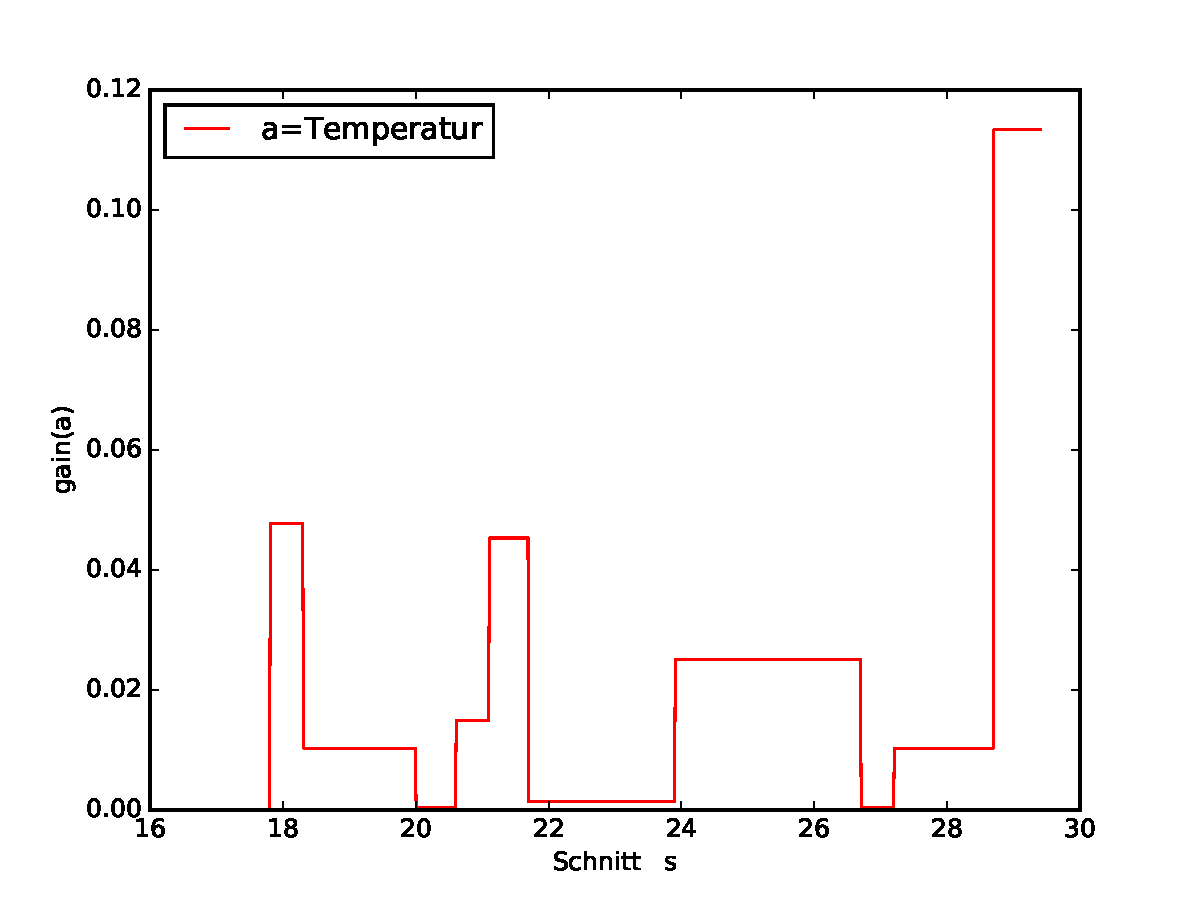
\includegraphics[width=0.7\textwidth]{Temperatur.pdf}
  \caption{ Der Informationsgewinn gain(a) in Abhängigkeit von dem Schnitt $s$ auf dem Attribut a=Luftfeuchigkeit .}
  \label{fig:Luftfeuchigkeit}
\end{figure}
\FloatBarrier


\subsection{d)}
\label{subsec:a3d}
Ein Schnitt s auf dem Attribut Temperatur liefert für
\begin{align}
 s=28,7
  \intertext{den größten Informationsgewinn gain(Temperatur) von:}
  \text{gain(a)} \approx 0,11
\end{align}
